\documentclass[11pt,a4paper]{article}

% ── Packages ──────────────────────────────────────────────────────────────────
\usepackage[utf8]{inputenc}
\usepackage[T1]{fontenc}
\usepackage{lmodern}
\usepackage[margin=2.5cm]{geometry}
\usepackage{amsmath, amssymb, amsthm}
\usepackage{graphicx}
\usepackage{booktabs}
\usepackage{enumitem}
\usepackage{hyperref}
\usepackage{fancyhdr}
\usepackage{xcolor}
\usepackage[most]{tcolorbox}
\usepackage{tikz}
\usetikzlibrary{arrows.meta, positioning, shapes.geometric}

% ── Colours ───────────────────────────────────────────────────────────────────
\definecolor{conceptbg}{RGB}{230,245,255}
\definecolor{conceptframe}{RGB}{70,130,180}
\definecolor{notebg}{RGB}{255,250,230}
\definecolor{noteframe}{RGB}{200,170,50}
\definecolor{errorbg}{RGB}{255,235,235}
\definecolor{errorframe}{RGB}{200,50,50}
\definecolor{correctbg}{RGB}{235,255,235}
\definecolor{correctframe}{RGB}{50,160,50}

% ── tcolorbox environments ────────────────────────────────────────────────────
\newtcolorbox{concept}[1][]{colback=conceptbg, colframe=conceptframe,
  fonttitle=\bfseries, title={#1}, sharp corners=south, boxrule=0.8pt}

\newtcolorbox{note}[1][]{colback=notebg, colframe=noteframe,
  fonttitle=\bfseries, title={#1}, sharp corners=south, boxrule=0.8pt}

\newtcolorbox{errorbox}[1][]{colback=errorbg, colframe=errorframe,
  fonttitle=\bfseries, title={#1}, sharp corners=south, boxrule=0.8pt}

\newtcolorbox{correctbox}[1][]{colback=correctbg, colframe=correctframe,
  fonttitle=\bfseries, title={#1}, sharp corners=south, boxrule=0.8pt}

% ── Headers ───────────────────────────────────────────────────────────────────
\pagestyle{fancy}
\fancyhf{}
\lhead{\small Teacher Guide: Conditional VAE}
\rhead{\small ETH -- Business \& Machine AI}
\cfoot{\thepage}

% ── Theorem environments ─────────────────────────────────────────────────────
\newtheorem{theorem}{Theorem}[section]
\newtheorem{proposition}[theorem]{Proposition}
\newtheorem{definition}[theorem]{Definition}

\hypersetup{
  colorlinks=true,
  linkcolor=conceptframe,
  urlcolor=conceptframe,
  citecolor=conceptframe
}

% ══════════════════════════════════════════════════════════════════════════════
\title{\textbf{Teacher Guide: Conditional Variational Autoencoders}\\[0.5em]
       \large Architecture, Theory, and Exercise Design\\[0.3em]
       \normalsize ETH -- Business \& Machine AI, FS26}
\author{Course Staff --- Internal Document}
\date{\today}

\begin{document}
\maketitle
\tableofcontents
\newpage

% ══════════════════════════════════════════════════════════════════════════════
\section{Overview}

This document provides an in-depth reference for the Conditional VAE (CVAE) in-class exercise. It covers the full mathematical derivation, architectural design decisions, file relationships, and pedagogical notes.

\begin{concept}[Exercise Objectives]
After completing this exercise, students should be able to:
\begin{enumerate}
    \item Explain the difference between AE, VAE, and CVAE architectures
    \item Implement the reparametrization trick and understand why it is necessary
    \item Build a conditional encoder/decoder that accepts auxiliary label information
    \item Train a CVAE and interpret the ELBO loss components
    \item Use a trained CVAE for conditional generation and latent interpolation
    \item Reason about the $\beta$ trade-off between reconstruction and regularisation
\end{enumerate}
\end{concept}

\subsection{Prerequisites}
Students should have completed the \textbf{Autoencoders CX} exercise and be familiar with:
\begin{itemize}
    \item Encoder-decoder architectures (convolutional)
    \item PyTorch basics: \texttt{nn.Module}, forward pass, training loops
    \item MSE loss, Adam optimiser, basic training diagnostics
\end{itemize}

\subsection{Estimated Duration}
45--60 minutes for the core TODOs (1--3). The full notebook including $\beta$ experiments takes approximately 75--90 minutes.

% ══════════════════════════════════════════════════════════════════════════════
\section{Theoretical Background}

\subsection{Generative Models and Latent Variables}

\begin{definition}[Latent Variable Model]
A latent variable model assumes observed data $\mathbf{x}$ is generated by first sampling an unobserved (latent) variable $\mathbf{z}$ from a prior $p(\mathbf{z})$, then generating $\mathbf{x}$ from a conditional distribution $p_\theta(\mathbf{x} | \mathbf{z})$:
\[
p_\theta(\mathbf{x}) = \int p_\theta(\mathbf{x} | \mathbf{z})\, p(\mathbf{z})\, d\mathbf{z}
\]
\end{definition}

The integral is intractable for complex models (neural networks), which motivates variational inference.

\subsection{Variational Autoencoders (VAE)}

\subsubsection{The Evidence Lower Bound (ELBO)}

We want to maximise $\log p_\theta(\mathbf{x})$ but cannot compute it directly. Introducing an approximate posterior $q_\phi(\mathbf{z} | \mathbf{x})$ (the encoder):

\begin{theorem}[ELBO Derivation]
\begin{align}
\log p_\theta(\mathbf{x}) &= \log \int p_\theta(\mathbf{x} | \mathbf{z})\, p(\mathbf{z})\, d\mathbf{z} \\
&= \log \int \frac{q_\phi(\mathbf{z}|\mathbf{x})}{q_\phi(\mathbf{z}|\mathbf{x})} p_\theta(\mathbf{x}|\mathbf{z})\, p(\mathbf{z})\, d\mathbf{z} \\
&\geq \int q_\phi(\mathbf{z}|\mathbf{x}) \log \frac{p_\theta(\mathbf{x}|\mathbf{z})\, p(\mathbf{z})}{q_\phi(\mathbf{z}|\mathbf{x})}\, d\mathbf{z} \quad \text{(Jensen's inequality)} \\
&= \underbrace{\mathbb{E}_{q_\phi(\mathbf{z}|\mathbf{x})}\left[\log p_\theta(\mathbf{x}|\mathbf{z})\right]}_{\text{Reconstruction term}} - \underbrace{D_{\mathrm{KL}}\left(q_\phi(\mathbf{z}|\mathbf{x}) \| p(\mathbf{z})\right)}_{\text{Regularisation term}}
\end{align}
This is the \textbf{Evidence Lower Bound (ELBO)}.
\end{theorem}

The gap between $\log p_\theta(\mathbf{x})$ and the ELBO is exactly $D_{\mathrm{KL}}(q_\phi(\mathbf{z}|\mathbf{x}) \| p_\theta(\mathbf{z}|\mathbf{x}))$, which is always non-negative. Maximising the ELBO simultaneously:
\begin{itemize}
    \item Pushes the decoder to reconstruct well (reconstruction term)
    \item Pushes the encoder to match the prior $p(\mathbf{z}) = \mathcal{N}(\mathbf{0}, \mathbf{I})$ (KL term)
\end{itemize}

\subsubsection{Closed-Form KL for Gaussians}

When $q_\phi(\mathbf{z}|\mathbf{x}) = \mathcal{N}(\boldsymbol{\mu}, \mathrm{diag}(\boldsymbol{\sigma}^2))$ and $p(\mathbf{z}) = \mathcal{N}(\mathbf{0}, \mathbf{I})$:

\begin{concept}[KL Divergence (Gaussian)]
\[
D_{\mathrm{KL}}\left(q_\phi \| p\right) = -\frac{1}{2} \sum_{j=1}^{d} \left(1 + \log \sigma_j^2 - \mu_j^2 - \sigma_j^2\right)
\]
In practice, the encoder outputs $\log \sigma^2$ (log-variance) for numerical stability:
\[
D_{\mathrm{KL}} = -\frac{1}{2} \sum_{j=1}^{d} \left(1 + \log\text{var}_j - \mu_j^2 - e^{\log\text{var}_j}\right)
\]
\end{concept}

\subsubsection{The Reparametrization Trick}

\begin{concept}[Why Reparametrize?]
The encoder defines a distribution $q_\phi(\mathbf{z}|\mathbf{x})$, and we need to sample $\mathbf{z}$ from it during training. However, the \texttt{sample()} operation has no gradient. The reparametrization trick makes sampling differentiable:
\[
\mathbf{z} = \boldsymbol{\mu}_\phi(\mathbf{x}) + \boldsymbol{\sigma}_\phi(\mathbf{x}) \odot \boldsymbol{\varepsilon}, \quad \boldsymbol{\varepsilon} \sim \mathcal{N}(\mathbf{0}, \mathbf{I})
\]
Now $\mathbf{z}$ is a deterministic function of $\phi$ (and random $\varepsilon$), so gradients $\nabla_\phi$ flow through $\boldsymbol{\mu}$ and $\boldsymbol{\sigma}$.
\end{concept}

\subsection{Conditional Variational Autoencoders (CVAE)}

\subsubsection{Motivation}

A standard VAE models $p(\mathbf{x})$ — it can generate data but has no control over \emph{what} it generates. A CVAE models $p(\mathbf{x} | \mathbf{c})$ where $\mathbf{c}$ is a condition (e.g., digit label, face attributes):

\begin{definition}[Conditional VAE]
A CVAE extends the VAE by conditioning all distributions on an observed variable $\mathbf{c}$:
\begin{itemize}
    \item \textbf{Encoder}: $q_\phi(\mathbf{z} | \mathbf{x}, \mathbf{c})$ --- infers latent representation given \emph{both} data and condition
    \item \textbf{Decoder}: $p_\theta(\mathbf{x} | \mathbf{z}, \mathbf{c})$ --- generates data given latent code and condition
    \item \textbf{Prior}: $p(\mathbf{z} | \mathbf{c})$ --- prior over latent space (often assumed label-independent: $p(\mathbf{z}) = \mathcal{N}(\mathbf{0}, \mathbf{I})$)
\end{itemize}
\end{definition}

\subsubsection{CVAE ELBO}

\begin{theorem}[Conditional ELBO]
\[
\log p_\theta(\mathbf{x} | \mathbf{c}) \geq \mathbb{E}_{q_\phi(\mathbf{z}|\mathbf{x},\mathbf{c})}\left[\log p_\theta(\mathbf{x} | \mathbf{z}, \mathbf{c})\right] - D_{\mathrm{KL}}\left(q_\phi(\mathbf{z}|\mathbf{x},\mathbf{c}) \| p(\mathbf{z}|\mathbf{c})\right)
\]
Assuming $p(\mathbf{z}|\mathbf{c}) = p(\mathbf{z}) = \mathcal{N}(\mathbf{0}, \mathbf{I})$ (label-independent prior), the KL term is identical to the standard VAE.
\end{theorem}

\begin{note}[Label-Independent Prior]
The assumption $p(\mathbf{z}|\mathbf{c}) = \mathcal{N}(\mathbf{0}, \mathbf{I})$ means that the prior distribution of ``style'' is the same regardless of the digit class. This is a simplification --- in principle, one could learn class-dependent priors $p(\mathbf{z}|\mathbf{c})$, but the standard assumption works well in practice and simplifies training.
\end{note}

\subsubsection{How Conditioning Changes the Architecture}

The key architectural difference between a VAE and a CVAE is \emph{where} and \emph{how} the condition $\mathbf{c}$ is injected:

\begin{concept}[Conditioning Mechanisms]
\textbf{Encoder conditioning (spatial broadcast):}
\begin{enumerate}
    \item One-hot label $\mathbf{c} \in \{0,1\}^{10}$ is reshaped to $(10, 1, 1)$
    \item Broadcast to match image spatial dimensions: $(10, 28, 28)$
    \item Concatenated with image along channel dimension: $(1, 28, 28) \oplus (10, 28, 28) = (11, 28, 28)$
\end{enumerate}
This gives every spatial location access to the label information, allowing the convolutional layers to learn label-dependent features from the first layer.

\textbf{Decoder conditioning (vector concatenation):}
\begin{enumerate}
    \item Sampled $\mathbf{z} \in \mathbb{R}^{32}$ is concatenated with $\mathbf{c} \in \mathbb{R}^{10}$
    \item Combined vector $[\mathbf{z}; \mathbf{c}] \in \mathbb{R}^{42}$ is fed to the decoder
\end{enumerate}
This is simpler than the encoder approach because the decoder starts from a vector (not a spatial feature map).
\end{concept}

\begin{note}[Alternative Conditioning Strategies]
Other approaches exist:
\begin{itemize}
    \item \textbf{Adaptive Instance Normalisation (AdaIN)}: condition modulates BN parameters (used in StyleGAN)
    \item \textbf{Cross-attention}: condition attends to features (used in Stable Diffusion)
    \item \textbf{FiLM}: condition produces scale and shift for feature maps
\end{itemize}
For this exercise, we use the simplest approach (concatenation) from the original CVAE paper (Sohn et al., 2015).
\end{note}

\subsection{The $\beta$-VAE Framework}

\begin{concept}[$\beta$-VAE (Higgins et al., 2017)]
The generalised ELBO with a hyperparameter $\beta$:
\[
\mathcal{L}_\beta = \mathbb{E}_{q_\phi(\mathbf{z}|\mathbf{x},\mathbf{c})}\left[\log p_\theta(\mathbf{x}|\mathbf{z},\mathbf{c})\right] - \beta \cdot D_{\mathrm{KL}}\left(q_\phi(\mathbf{z}|\mathbf{x},\mathbf{c}) \| p(\mathbf{z})\right)
\]
\begin{itemize}
    \item $\beta = 1$: standard VAE (ELBO)
    \item $\beta < 1$: weaker regularisation $\Rightarrow$ sharper reconstructions, less structured latent space
    \item $\beta > 1$: stronger regularisation $\Rightarrow$ blurrier output, more disentangled latent representations
\end{itemize}
\end{concept}

From an information-theoretic perspective, $\beta$ controls the \textbf{rate-distortion trade-off}: higher $\beta$ limits the information flow through the bottleneck (rate), forcing the model to rely more on the prior (which may increase distortion).

\begin{errorbox}[Common Misconception]
Students often think $\beta > 1$ is always better because ``more regularisation = more structure''. In practice, excessively high $\beta$ causes \textbf{posterior collapse}: the encoder learns to ignore the input entirely, outputting $q(\mathbf{z}|\mathbf{x}) \approx p(\mathbf{z})$ for all $\mathbf{x}$. The decoder then ignores $\mathbf{z}$ and relies solely on the label, producing low-diversity outputs.
\end{errorbox}

% ══════════════════════════════════════════════════════════════════════════════
\section{Architecture Details}

\subsection{Overview}

\begin{center}
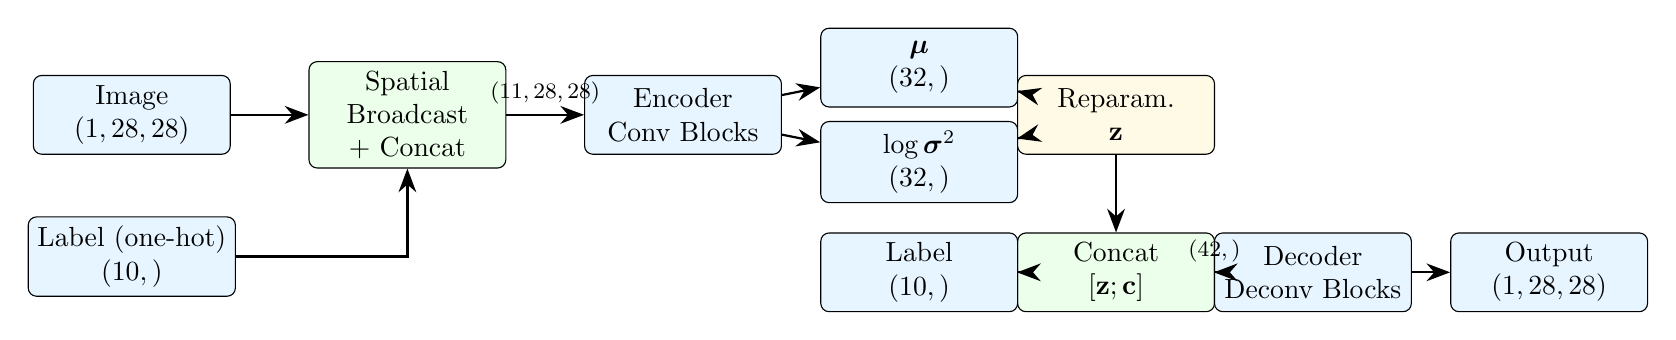
\begin{tikzpicture}[
    block/.style={rectangle, draw, fill=conceptbg, minimum width=2.5cm, minimum height=1cm, align=center, rounded corners=3pt},
    arrow/.style={-{Stealth[length=3mm]}, thick},
    label/.style={font=\footnotesize\itshape}
]
    % Encoder
    \node[block] (img) at (0,0) {Image\\$(1, 28, 28)$};
    \node[block] (lbl_e) at (0,-1.8) {Label (one-hot)\\$(10,)$};
    \node[block, fill=correctbg] (cond) at (3.5,0) {Spatial\\Broadcast\\+ Concat};
    \node[block] (enc) at (7,0) {Encoder\\Conv Blocks};
    \node[block] (mu) at (10,0.6) {$\boldsymbol{\mu}$\\$(32,)$};
    \node[block] (lv) at (10,-0.6) {$\log\boldsymbol{\sigma}^2$\\$(32,)$};

    % Reparametrize
    \node[block, fill=notebg] (reparam) at (12.5,0) {Reparam.\\$\mathbf{z}$};

    % Decoder
    \node[block, fill=correctbg] (concat) at (12.5,-2) {Concat\\$[\mathbf{z}; \mathbf{c}]$};
    \node[block] (lbl_d) at (10,-2) {Label\\$(10,)$};
    \node[block] (dec) at (15,-2) {Decoder\\Deconv Blocks};
    \node[block] (out) at (18,-2) {Output\\$(1, 28, 28)$};

    % Arrows
    \draw[arrow] (img) -- (cond);
    \draw[arrow] (lbl_e) -| (cond);
    \draw[arrow] (cond) -- node[above, label] {$(11, 28, 28)$} (enc);
    \draw[arrow] (enc) -- (mu);
    \draw[arrow] (enc) -- (lv);
    \draw[arrow] (mu) -- (reparam);
    \draw[arrow] (lv) -- (reparam);
    \draw[arrow] (reparam) -- (concat);
    \draw[arrow] (lbl_d) -- (concat);
    \draw[arrow] (concat) -- node[above, label] {$(42,)$} (dec);
    \draw[arrow] (dec) -- (out);
\end{tikzpicture}
\end{center}

\subsection{Encoder Architecture}

\begin{center}
\begin{tabular}{lllll}
\toprule
\textbf{Layer} & \textbf{Type} & \textbf{Config} & \textbf{Output Shape} & \textbf{Notes} \\
\midrule
Input & --- & --- & $(B, 11, 28, 28)$ & Image + broadcast label \\
Conv Block 1 & Conv2d + BN + LeakyReLU & $k\!=\!3$, $s\!=\!2$, $p\!=\!1$, $C\!=\!32$ & $(B, 32, 14, 14)$ & Stride 2 downsamples \\
Conv Block 2 & Conv2d + BN + LeakyReLU & $k\!=\!3$, $s\!=\!2$, $p\!=\!1$, $C\!=\!64$ & $(B, 64, 7, 7)$ & Stride 2 downsamples \\
Conv Block 3 & Conv2d + BN + LeakyReLU & $k\!=\!3$, $s\!=\!1$, $p\!=\!1$, $C\!=\!128$ & $(B, 128, 7, 7)$ & No downsampling \\
Flatten & --- & --- & $(B, 6272)$ & $128 \times 7 \times 7$ \\
\texttt{fc\_mu} & Linear & $6272 \to 32$ & $(B, 32)$ & Mean of $q(\mathbf{z}|\mathbf{x}, \mathbf{c})$ \\
\texttt{fc\_log\_var} & Linear & $6272 \to 32$ & $(B, 32)$ & Log-variance of $q(\mathbf{z}|\mathbf{x}, \mathbf{c})$ \\
\bottomrule
\end{tabular}
\end{center}

\subsection{Decoder Architecture}

\begin{center}
\begin{tabular}{lllll}
\toprule
\textbf{Layer} & \textbf{Type} & \textbf{Config} & \textbf{Output Shape} & \textbf{Notes} \\
\midrule
Input & --- & --- & $(B, 42)$ & $\mathbf{z}$ (32) + label (10) \\
\texttt{decoder\_fc} & Linear + LeakyReLU & $42 \to 6272$ & $(B, 6272)$ & Expand to spatial \\
Reshape & --- & --- & $(B, 128, 7, 7)$ & Ready for deconv \\
Deconv Block 1 & ConvT2d + BN + LeakyReLU & $k\!=\!3$, $s\!=\!1$, $p\!=\!1$, $C\!=\!64$ & $(B, 64, 7, 7)$ & No upsampling \\
Deconv Block 2 & ConvT2d + BN + LeakyReLU & $k\!=\!4$, $s\!=\!2$, $p\!=\!1$, $C\!=\!32$ & $(B, 32, 14, 14)$ & Stride 2 upsamples \\
Deconv Block 3 & ConvT2d + Sigmoid & $k\!=\!4$, $s\!=\!2$, $p\!=\!1$, $C\!=\!1$ & $(B, 1, 28, 28)$ & Stride 2 upsamples \\
\bottomrule
\end{tabular}
\end{center}

\begin{note}[Kernel Size 4 for Upsampling]
We use $k\!=\!4$ with $s\!=\!2$, $p\!=\!1$ for upsampling layers. This ensures exact doubling of spatial dimensions: $H_\text{out} = (H_\text{in} - 1) \times s - 2p + k = (7-1)\times 2 - 2 + 4 = 14$. Using $k\!=\!3$ with $s\!=\!2$ would require \texttt{output\_padding=1} to achieve the same result.
\end{note}

\subsection{Design Decisions: MNIST vs.\ CelebA}

\begin{center}
\begin{tabular}{lll}
\toprule
\textbf{Aspect} & \textbf{Original (CelebA)} & \textbf{Exercise (MNIST)} \\
\midrule
Image size & $64 \times 64 \times 3$ (RGB) & $28 \times 28 \times 1$ (Grayscale) \\
Condition & 40 binary attributes & 10-class one-hot \\
Latent dim & 128 & 32 \\
Encoder depth & 4 conv blocks (stride 2 each) & 3 conv blocks (2 with stride 2) \\
Decoder depth & 5 deconv blocks & 3 deconv blocks \\
Framework & TensorFlow 2.x & PyTorch \\
Training time & Hours (full CelebA) & Minutes (MNIST) \\
\bottomrule
\end{tabular}
\end{center}

The core concepts (conditioning, reparametrization, ELBO, $\beta$ trade-off) are \textbf{identical} --- only the scale differs.

% ══════════════════════════════════════════════════════════════════════════════
\section{File Relationships}

\begin{center}
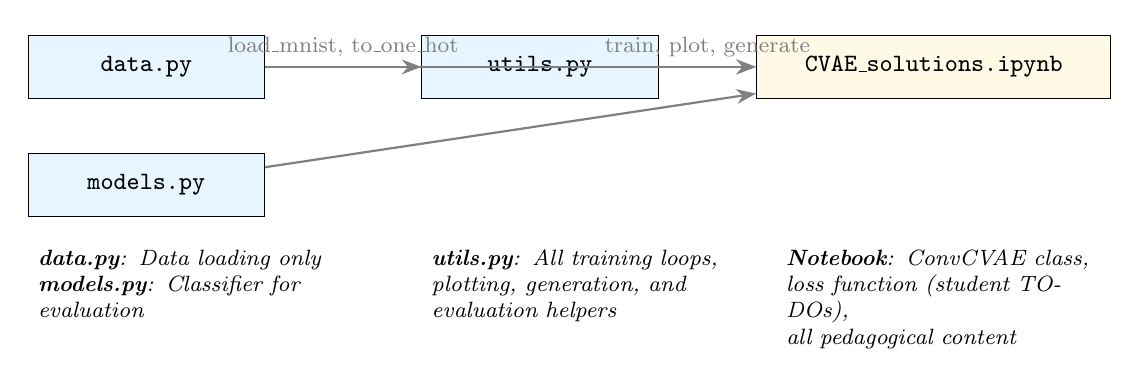
\begin{tikzpicture}[
    file/.style={rectangle, draw, fill=conceptbg, minimum width=3cm, minimum height=0.8cm, align=center, font=\ttfamily\small},
    arrow/.style={-{Stealth[length=2.5mm]}, thick, gray},
    note/.style={font=\footnotesize\itshape, text width=4cm, align=left}
]
    % Files
    \node[file] (data) at (0,0) {data.py};
    \node[file] (models) at (0,-1.5) {models.py};
    \node[file] (utils) at (5,0) {utils.py};
    \node[file, fill=notebg, minimum width=4.5cm] (nb) at (10,0) {CVAE\_solutions.ipynb};

    % Arrows
    \draw[arrow] (data) -- node[above, font=\footnotesize] {load\_mnist, to\_one\_hot} (utils);
    \draw[arrow] (data) -- (nb);
    \draw[arrow] (models) -- (nb);
    \draw[arrow] (utils) -- node[above, font=\footnotesize] {train, plot, generate} (nb);

    % Notes
    \node[note, anchor=north west] at (-1.5,-2.2) {
        \textbf{data.py}: Data loading only\\
        \textbf{models.py}: Classifier for evaluation
    };
    \node[note, anchor=north west] at (3.5,-2.2) {
        \textbf{utils.py}: All training loops,\\
        plotting, generation, and\\
        evaluation helpers
    };
    \node[note, anchor=north west] at (8,-2.2) {
        \textbf{Notebook}: ConvCVAE class,\\
        loss function (student TODOs),\\
        all pedagogical content
    };
\end{tikzpicture}
\end{center}

\subsection{Why the Model Lives in the Notebook}

Following the Autoencoders CX pattern, the \texttt{ConvCVAE} class and \texttt{cvae\_loss} function are defined \emph{in the notebook} rather than in a support file. This ensures:
\begin{itemize}
    \item Students see and modify the model directly
    \item The TODO structure is clear and self-contained
    \item No need to switch between files during the exercise
\end{itemize}

\subsection{Function Reference}

\begin{center}
\small
\begin{tabular}{llp{7cm}}
\toprule
\textbf{File} & \textbf{Function} & \textbf{Description} \\
\midrule
\texttt{data.py} & \texttt{load\_mnist()} & Downloads MNIST, returns numpy arrays normalised to $[0,1]$ \\
& \texttt{to\_one\_hot(y, n)} & Converts integer labels to one-hot float32 \\
\midrule
\texttt{models.py} & \texttt{MNISTClassifier} & CNN classifier for evaluating generation quality \\
\midrule
\texttt{utils.py} & \texttt{setup()} & Confirms device (CPU/GPU) \\
& \texttt{train\_classifier()} & Trains MNISTClassifier on labelled data \\
& \texttt{train\_cvae()} & Main CVAE training loop (Adam + cosine schedule) \\
& \texttt{plot\_losses()} & Plots total/recon/KL loss curves \\
& \texttt{reconstruct\_cvae()} & Forward pass, returns numpy reconstructions \\
& \texttt{plot\_original\_vs\_reconstructed()} & Side-by-side comparison plot \\
& \texttt{plot\_per\_digit\_mse()} & Per-digit reconstruction error analysis \\
& \texttt{generate\_conditional()} & Sample $\mathbf{z}$ + label $\to$ generate and display \\
& \texttt{generate\_digit\_grid()} & 10$\times$N grid of generated digits \\
& \texttt{interpolate\_latent()} & Latent space interpolation with optional label switch \\
& \texttt{visualise\_latent\_space\_cvae()} & PCA scatter of $\boldsymbol{\mu}$ coloured by digit \\
& \texttt{evaluate\_and\_plot\_confusion()} & Classifier accuracy + confusion matrix \\
& \texttt{evaluate\_generated\_images()} & Generate per-digit, classify, report accuracy \\
\midrule
\texttt{notebook} & \texttt{ConvCVAE} & The CVAE model class (student TODOs) \\
& \texttt{cvae\_loss()} & ELBO loss function (student TODO) \\
\bottomrule
\end{tabular}
\end{center}

% ══════════════════════════════════════════════════════════════════════════════
\section{TODO Solutions and Grading Notes}

\subsection{TODO 1: ConvCVAE Methods}

\begin{correctbox}[TODO 1a: \texttt{conditional\_input}]
\begin{verbatim}
def conditional_input(self, x, label):
    label_map = label.unsqueeze(-1).unsqueeze(-1)
    label_map = label_map.expand(-1, -1, x.size(2), x.size(3))
    return torch.cat([x, label_map], dim=1)
\end{verbatim}
\textbf{Key point:} Students must understand broadcasting. Common error: trying to use \texttt{label.view(B, 10, 28, 28)} directly (wrong --- that reshapes rather than broadcasts).
\end{correctbox}

\begin{correctbox}[TODO 1b: \texttt{reparametrize}]
\begin{verbatim}
def reparametrize(self, mu, log_var):
    std = torch.exp(0.5 * log_var)
    eps = torch.randn_like(std)
    return mu + std * eps
\end{verbatim}
\textbf{Key point:} Must use \texttt{log\_var * 0.5} (not \texttt{log\_var ** 0.5}). The encoder outputs \emph{log-variance}, not variance.
\end{correctbox}

\begin{correctbox}[TODO 1c--e: \texttt{encode}, \texttt{decode}, \texttt{forward}]
These are straightforward sequential compositions. Common errors:
\begin{itemize}
    \item Forgetting \texttt{.flatten(1)} between conv and fc layers
    \item Wrong reshape dimensions in \texttt{decode} (must be $128 \times 7 \times 7$)
    \item Forgetting to concatenate label in \texttt{decode}
\end{itemize}
\end{correctbox}

\subsection{TODO 2: Loss Function}

\begin{correctbox}[TODO 2a--b: BCE + KL]
\begin{verbatim}
recon_loss = F.binary_cross_entropy(recon_x, x, reduction='sum') / batch_size
kl_loss = -0.5 * torch.sum(1 + log_var - mu.pow(2) - log_var.exp()) / batch_size
\end{verbatim}
\textbf{Key point:} Students may confuse \texttt{reduction='sum'} vs \texttt{'mean'}. We sum over pixels then average over batch for consistency with the KL term.
\end{correctbox}

\subsection{TODOs 3--5: Open-Ended Exploration}

These are not graded for correctness but for engagement. Look for:
\begin{itemize}
    \item TODO 3: Did they try multiple digits? Did they notice style variation?
    \item TODO 4: Did they compare fixed-label vs.\ label-switch interpolation?
    \item TODO 5: Did they articulate the $\beta$ trade-off?
\end{itemize}

% ══════════════════════════════════════════════════════════════════════════════
\section{Expected Student Difficulties}

\begin{errorbox}[Difficulty 1: ``Why is the VAE blurrier than the AE?'']
The KL term prevents the encoder from using the full capacity of the latent space. This is by design --- it creates a smooth latent space that enables generation. The AE has no such constraint, so it can achieve lower reconstruction error at the cost of a ``holey'' latent space.
\end{errorbox}

\begin{errorbox}[Difficulty 2: Shape Errors in \texttt{conditional\_input}]
The spatial broadcast of labels is conceptually simple but easy to get wrong. Students may try \texttt{label.repeat(1, 1, 28, 28)} (wrong --- repeat duplicates along existing dims, doesn't add new ones). The correct pattern is \texttt{unsqueeze} then \texttt{expand}.
\end{errorbox}

\begin{errorbox}[Difficulty 3: ``Why does the latent space overlap more?'']
Students who completed the AE exercise expect clear digit clusters. In a CVAE, the label carries identity, so $\mathbf{z}$ captures shared style features. More overlap = better disentanglement. Frame this as a \emph{feature}, not a bug.
\end{errorbox}

\begin{errorbox}[Difficulty 4: KL Loss Going Up]
Students may be alarmed that KL loss increases during training. Explain: at initialisation, the encoder outputs near-zero $\mu$ and $\log\sigma^2$, so KL $\approx 0$. As the encoder learns to encode information in $\mathbf{z}$, KL increases. It should eventually plateau.
\end{errorbox}

% ══════════════════════════════════════════════════════════════════════════════
\section{Discussion Points for Class}

\begin{enumerate}
    \item \textbf{AE vs.\ CVAE latent spaces:} Why does the CVAE latent space show more overlap between digit classes? Is this desirable?

    \item \textbf{Continuous conditions:} What if instead of a digit label, we conditioned on a continuous variable (e.g., rotation angle)? How would the architecture change?

    \item \textbf{Connection to diffusion models:} Modern text-to-image models (Stable Diffusion, DALL-E) also use conditioning. How is their approach similar to / different from a CVAE?

    \item \textbf{The CelebA version:} The original project used 40 binary face attributes. What new capabilities does this enable? (Attribute manipulation: ``add glasses'', ``change hair colour'' while preserving identity.)

    \item \textbf{Posterior collapse:} What happens with very high $\beta$? The encoder may learn to ignore the input entirely (``posterior collapse''). How would you detect this?

    \item \textbf{Label-dependent priors:} We assumed $p(\mathbf{z}) = \mathcal{N}(\mathbf{0}, \mathbf{I})$ for all labels. What if different digits have different priors? Would this help or hurt?
\end{enumerate}

% ══════════════════════════════════════════════════════════════════════════════
\section{References}

\begin{enumerate}
    \item Kingma, D.P. \& Welling, M. (2014). \textit{Auto-Encoding Variational Bayes}. ICLR.
    \item Sohn, K., Lee, H., \& Yan, X. (2015). \textit{Learning Structured Output Representation using Deep Conditional Generative Models}. NeurIPS.
    \item Higgins, I. et al. (2017). \textit{$\beta$-VAE: Learning Basic Visual Concepts with a Constrained Variational Framework}. ICLR.
    \item Doersch, C. (2016). \textit{Tutorial on Variational Autoencoders}. arXiv:1606.05908.
\end{enumerate}

\end{document}
